\section{The Parabolic Anchor Compiler}
% =====================================================================
The anchor vector $a=(a_u,a_d,a_e)=(1,1,2)$ --- the absolute value of the splitting type
$\mathcal O(-1)\oplus\mathcal O(-1)\oplus\mathcal O(-2)$ --- is the smallest parabolic object that
encodes the three operative structures at once:
\begin{equation}
  \boxed{\ \|a\|_1=1{+}1{+}2=4=|\mu_4|=-\deg E,\quad
  \|a\|_2^2=1{+}1{+}4=6=|R^+(A_3)|,\quad
  \textstyle\prod_i a_i=2=|\mathbb Z_2|_{\text{sheet}}\ }\ \mE .
\end{equation}
The $\ell^1$ norm is the glue/anti-degree, the $\ell^2$ norm$^2$ is the $A_3$ positive-root hexagon, and
the product is the sheet parity.

\subsection{Budget master table: everything is $d_p=-\deg E=4$ times a Coxeter datum}
With $d_p:=-\deg E=4$ fixed by parabolic degree zero, the entire integer landscape collapses:
\begin{equation}
\boxed{\ \setlength{\arraycolsep}{2pt}\begin{aligned}
  \textstyle\sum_{f,j}L_{f,j}&=d_p\,\AL=40, & 10b_1&=1+d_p\,\AL=41, \\
  \Oadm&=d_p\,|R(A_3)|=48, & \Dstart&=d_p\dim A_3=60, \\
  \operatorname{Tr}_{S^+}X^2&=d_p\,h=120, & |R(E_8)|&=2d_p\,h=240, \\
  \dim E_8&=d_p\,h+2d_p\dim S^+=248, & 128&=2\dim S^+(-\deg E).
\end{aligned}\ }\ \mE
\end{equation}
So $40,41,48,60,120,240,248$ and the spinor block $128$ are all functions of
\[(d_p,\AL,|R(A_3)|,\dim A_3,h,\dim S^+)=(4,10,12,15,30,16),\]
with the single new ingredient $d_p=4$ \emph{derived} from parabolic degree zero (not posited).

\subsection{Flavor budget split, row sums, scalaron deficit}
The flavor budget splits into anchor $+$ two equal Coxeter copies:
\begin{equation}
  \boxed{\ \textstyle\sum_{f,j}L_{f,j}=\|a\|_1+2\Nfam|R^+(A_3)|=4+2\cdot3\cdot6=40=\underbrace{4}_{\text{anchor}}+\underbrace{18}_{\text{winding}}+\underbrace{18}_{\text{non-anchor residue}}\ }\qquad\mE .
\end{equation}
The residue row sums and full row sums read named objects,
\begin{equation}
\begin{aligned}
  &(R_u,R_d,R_e)=(4,8,10)=(|\mu_4|,\,h(D_5),\,\AL),\\
  &(\textstyle\sum L_u,\sum L_d,\sum L_e)=(10,14,16)=(\AL,\,h(D_5)+|R^+(A_3)|,\,\dim S^+),
\end{aligned}
\end{equation}
and the generation (column) sums are
$(G_1,G_2,G_3)=(\|a\|_1+\Nfam|R^+(A_3)|,\,|R(A_3)|+N_\Phi,\,\gcar)=(4{+}18,\,12{+}1,\,5)=(22,13,5)$. \mE\
Finally the scalaron exponent is the parabolic anti-degree plus the family rank,
\begin{equation}
  \boxed{\ \frac{M_{\mathrm{scal}}^2}{\Mbar^2}=\cthree^{\,-\deg E+\operatorname{rk}E}=\cthree^{\,4+3}=\cthree^7\ }\qquad\mE\ \veri{v7\_gravity\_cosmo.py} ,
\end{equation}
linking the stable family bundle $\mathcal O(-2)\oplus\mathcal O(-1)^2$ directly to the inflation scale.
The $\mathbb Z_6$ residue sum is the projected parabolic count
$\sum r=2\sum c+3\sum s-|R(A_3)|=2h(D_5)+3|R^+(A_3)|-|R(A_3)|=16+18-12=22=h_{E_8}-r_{E_8}$,
the two overflows of $6$ being exactly $|R(A_3)|=12$. \mE

\subsection{The anchor power compiler}

\begin{figure}[h]\centering
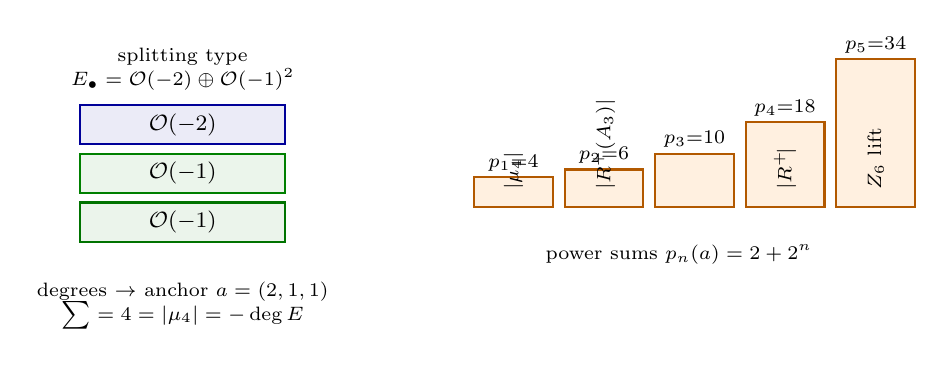
\begin{tikzpicture}[font=\footnotesize]
% splitting type bundle
\begin{scope}
  \foreach \i/\d/\c in {0/{-2}/blue!60!black, 1/{-1}/green!50!black, 2/{-1}/green!45!black}{
     \draw[thick,\c,fill=\c!8] (0,-\i*0.62) rectangle (2.6,-\i*0.62+0.5);
     \node at (1.3,-\i*0.62+0.25) {$\mathcal O(\d)$};}
  \node[align=center] at (1.3,0.95) {\scriptsize splitting type\\[-1pt]\scriptsize $E_\bullet=\mathcal O(-2)\oplus\mathcal O(-1)^2$};
  \node[align=center] at (1.3,-2.05) {\scriptsize degrees $\to$ anchor $a=(2,1,1)$\\[-1pt]\scriptsize $\sum=4=|\mu_4|=-\deg E$};
\end{scope}
% power sum ladder
\begin{scope}[shift={(5.0,-0.8)}]
  \foreach \n/\v/\lab in {1/4/{$|\mu_4|$},2/6/{$|R^+(A_3)|$},3/10/{$\AL$},4/18/{$\Nfam|R^+\!|$},5/34/{$\mathbb Z_6$ lift}}{
     \draw[thick,orange!70!black,fill=orange!12] ({(\n-1)*1.15},0) rectangle ({(\n-1)*1.15+1.0},{0.18+\v*0.05});
     \node[font=\scriptsize] at ({(\n-1)*1.15+0.5},{0.18+\v*0.05+0.18}) {$p_{\n}{=}\v$};
     \node[font=\scriptsize,rotate=90,anchor=west] at ({(\n-1)*1.15+0.5},0.1) {\lab};}
  \node[align=center] at (2.6,-0.6) {\scriptsize power sums $p_n(a)=2+2^n$};
\end{scope}
\end{tikzpicture}
\caption{\small The $(1,1,2)$ microcode. Left: the parabolic-stable splitting type
$\mathcal O(-2)\oplus\mathcal O(-1)^2$ whose degrees are the anchor. Right: its power sums
$p_n=2+2^n=(4,6,10,18,34)$ generate $|\mu_4|$, $|R^+(A_3)|$, the decuple $\AL$, and the whole budget.}
\end{figure}

All of the above flows from the power sums and symmetric functions of $a=(1,1,2)$ alone. The power
sums are $p_n(a)=\sum_i a_i^n=2+2^n$:
\begin{equation}
  \boxed{\ (p_1,p_2,p_3,p_4,p_5)=(4,6,10,18,34)=\bigl(|\mu_4|,\,|R^+(A_3)|,\,\AL,\,\Nfam|R^+(A_3)|,\,\text{raw }\mathbb Z_6\text{ lift}\bigr)\ }\qquad\mE ,
\end{equation}
so the decuple is the \emph{cubic} anchor moment $\AL=p_3=1{+}1{+}8=10$. The elementary symmetric
functions ($\chi_a(t)=(t-1)^2(t-2)=t^3-4t^2+5t-2$) are
\begin{equation}
  \boxed{\ e_1=4=|\mu_4|,\quad e_2=5=\gcar,\quad e_3=2=|\mathbb Z_2|,\qquad p_0^2+e_1^2=3^2+4^2=5^2=e_2^2\ }\qquad\mE ,
\end{equation}
so the flavor anchor \emph{reconstructs the carrier rank} $\gcar=e_2(a)=5$, and the $3,4,5$ triangle
sits inside it; the $U(1)$ integer is $10b_1=e_1^2+e_2^2=1+p_1p_3=41$. The glue norms and the whole
budget table are power-sum ratios/products:
\begin{equation}
\begin{aligned}
  &q(A_3)=\frac{p_2}{2p_1}=\frac34,\quad q(D_5)=\frac{p_3}{2p_1}=\frac54;\\
  &\sum L=p_1p_3,\ \Oadm=2p_1p_2,\ \Dstart=p_2p_3,\ \operatorname{Tr}_{S^+}X^2=2p_2p_3,\ |R(E_8)|=4p_2p_3,
\end{aligned}
\end{equation}
with $h=\tfrac{p_2p_3}{2}=30$, $r=2p_1=8$, $\dim S^+=2^{p_1}=16$, $\dim E_8=2p_2p_3+2^{p_1+1}p_1=248$,
and the seed $\useed=\tfrac{2p_1}{p_2}\cthree+2p_1p_2\cthree^4$. The scalaron exponent has the equivalent
readings $7=p_0+p_1=\Nfam+|\mu_4|=e_2+e_3=\gcar+|\mathbb Z_2|=h(D_5)-1=\dim A_3-h(D_5)=\Oadm-10b_1$. \mE

\subsection{Residue-matrix spectral selector --- sharpening (H2)}
Hypotheses (H1),(H3) plus the unique sum-$4$ set fix the up and lepton sectors and reduce (H2) to a
\emph{single binary choice} in the down sector: $\{1,2,5\}$ versus its distinct-distance sibling
$\{1,3,4\}$ (both contain the anchor $1$, both have row sum $8$, so sum rules do not separate them). The
residue matrix $R$ (rows $u,d,e$; columns gen $1,2,3$) and its winding completion $L=R+6\,\mathbf 1 e_1^{\!\top}$
separate them by their \emph{spectral invariants}:
\begin{equation}
  R=\begin{pmatrix}1&3&0\\1&5&2\\2&5&3\end{pmatrix}:\quad
  \boxed{\ \operatorname{tr}R=9=\Nfam^2,\ \det R=8=h(D_5),\ \chi_R(t)=t^3-\Nfam^2t^2+\AL\,t-h(D_5)\ }\ \mE ,
\end{equation}
\begin{equation}
  \boxed{\ \text{principal $2$-minors}(R)=(2,3,5)=(\text{sheet},\,\Nfam,\,\gcar),\quad
  \text{their }\textstyle\sum=10=\AL,\ \prod=30=h_{E_8}\ }\qquad\mE ,
\end{equation}
so the three TFPT atoms $2,3,5$ are literally the principal minors of the flavor residue matrix, and
$\|R\|_F^2=78=\dim E_6$ (an $E_6$ residue-shadow fingerprint \mO), $\operatorname{SNF}(R)=\operatorname{diag}(1,1,8)$.
The full length matrix has $\chi_L(t)=t^3-\dim(A_3)\,t^2+|R(D_5)|\,t-2\AL=t^3-15t^2+40t-20$, principal
minors $(5,14,21)=(\gcar,7\!\cdot\!2,7\!\cdot\!3)$, $\det L=20=|R(A_4)|=2\AL$, and
$\operatorname{SNF}(L)=\operatorname{diag}(1,1,20)$. The winding response is
$R^{-1}\mathbf 1=\tfrac14(1,1,-1)^{\!\top}$, i.e.\ $e_1^{\!\top}R^{-1}\mathbf 1=\tfrac1{|\mu_4|}$, giving
$\det L=\det R\,(1+6/|\mu_4|)=8\cdot\tfrac52=20$. The wrong sibling $\{1,3,4\}$ fails \emph{every} one of
these (it gives $\operatorname{tr}R'=8$, $\det R'=6$, minors $(-3,1,3)$, $\|R'\|_F^2=74$, $\det L'=-12$).

\begin{keybox}[The bidirectional anchor checksum (2026-08-07) --- one anchor decodes both sides, $1$ of $12$ \mE\ (\veri{v832\_anchor\_flavor\_checksum.py})]
The spectral-selector block and the bilinear table compress to \emph{one} statement: $R$ decodes the
\emph{same} anchor $a=(1,1,2)$ on both sides,
\[
  \boxed{\ Ra=(4,10,13)=(p_1,\,p_3,\,N(3{+}2i)),\qquad
  R^{\mathsf T}a=(6,18,8)=(p_2,\,p_4,\,p_3{-}2)\ }\qquad\mE ,
\]
rows reading the odd power sums plus the Gaussian norm $13=N(3{+}2i)=\Delta_Q$ (\vref{v222},
\vref{v230}, \vref{v415}) and columns reading the even power sums plus $8=h(D_5)$ --- the union covers
$p_1..p_4$ exactly.  \emph{The kill test is selective:} of the $12$ down-row candidates (all orderings
of the accepted $\{1,2,5\}$ and of the sibling $\{1,3,4\}$) exactly \emph{one} --- the accepted
$(1,5,2)$ --- satisfies the full identity set $\{\operatorname{tr},\det,\text{minors},\chi_R,Ra,
R^{\mathsf T}a\}$; no sibling ordering and no re-ordering of $\{1,2,5\}$ survives.  The new
one-number discriminator is the anchor contraction
\[
  (Ra)_2=\text{row}\cdot a=1{+}5{+}4=10=p_3=\AL,\qquad\text{siblings: }11\ \text{and}\ 12 ,
\]
so the down branch is killed by a single inner product against the anchor.  Controls: the scrambled
accepted ordering $(5,1,2)$ fails, and the sibling $(1,4,3)$ reproduces the failure numbers of the
block above verbatim.  A compression of the selector and bilinear tables ($15/15$ exact, verdict
\textsc{flavor-bidir-checksum} (selective)); no marker moves.
\end{keybox}

\smallskip
\noindent\textbf{More fingerprints (all verified).} The char-polynomials differ by an $A_3^+$ winding,
$\chi_L(t)-\chi_R(t)=-6(t^2-5t+2)=-|R^+(A_3)|\,(t^2-\gcar t+\mathbb Z_2)$. The inverse responses read the
two natural denominators, $R^{-1}\mathbf 1=\tfrac1{|\mu_4|}(1,1,-1)$ and
$L^{-1}\mathbf 1=\tfrac1{\AL}(1,1,-1)=\tfrac1{10}(1,1,-1)$ (glue denominator $4$ vs decuple denominator
$10$). The bilinear forms on $\{\mathbf 1,a\}$ with $a=(1,1,2)$ are
\begin{equation}
  \begin{array}{c|cc}
  R & \mathbf 1 & a\\\hline
  \mathbf 1^{\!\top} & 22=h{-}r & 27=3^3\\
  a^{\!\top} & 32=2^{\gcar} & 40=|R(D_5)|
  \end{array}
  \qquad\quad
  \begin{array}{c|cc}
  L & \mathbf 1 & a\\\hline
  \mathbf 1^{\!\top} & 40 & 45=\dim D_5\\
  a^{\!\top} & 56=7h(D_5) & 64=\dim S^+|\mu_4|
  \end{array}
\end{equation}
so $a^{\!\top}La=64=\dim S^+|\mu_4|$ is exactly one $E_8$ spinor glue sheet $(16,4)$, and the winding lift
$a^{\!\top}La-a^{\!\top}Ra=64-40=24=|W(A_3)|$ is the $A_3$ Weyl group. \mE
\par\smallskip\noindent\textbf{(H2), now a small algebraic selector --- and an honest negative result.}
With (H1),(H3), the cusp input (H2) is reduced to one binary branch, selected by the canonical spectral
form $\det R=h(D_5)$, principal minors $(2,3,5)$, $\chi_R=t^3-\Nfam^2t^2+\AL t-h(D_5)$. So ``derive the
flavor matrix from cusp geometry'' becomes the sharp statement: \emph{the cusp action on
$\mathbb P^1\setminus\mu_4$ realises the branch whose residue matrix has this canonical spectrum}.

\smallskip
\noindent\textbf{A tempting shortcut fails (verified).} One might hope the sector residue set is simply
the base triple reflected through the sector's cusp hexagon position $p_f=6\kappa_f\bmod 6$
($u\!\to\!4,d\!\to\!2,e\!\to\!0$). It is \emph{not}: that naive rule gives $\{1,2,5\}$ for up,
$\{1,3,4\}$ for down (the spectrally-\emph{failing} sibling!), $\{0,3,5\}$ for lepton --- wrong in all
three. The correct $D_6$ elements are $u=\mathrm{id}$, $e=\text{rot}+2$, $d=\text{reflection through }x{=}1$
(not through the cusp $x{=}2$); up and lepton are rotations while down is a reflection, so the three
sectors are not one clean cusp-rotation orbit. Hence H2 has \emph{no one-line cusp-position shortcut}.

\smallskip
\noindent\textbf{But H2 is not a free input: the transport-kernel theorem derives it.} The transport-kernel theorem
(``canonical transport kernel and single-winding closure'') fixes the residue packets from the
\emph{uniquely determined} rigid family connection $[\nabla_F^\star]$, its intrinsic holonomy
$\operatorname{Hol}_{\mathcal G_{D_4}}(\nabla_F^\star)$ on the $D_4$-invariant geodesic spine, the
structural transport kernel $K_f^{\mathrm{str}}$, and the resonance pole $\dph\in(\tfrac13,\tfrac23)$.
Its output is exactly $R_u=\{0,1,3\}$, $R_d=\{1,2,5\}$, $R_e=\{2,3,5\}$ --- the spectral-selector branch
($\det R=h(D_5)=8$, principal minors $(2,3,5)$), \emph{not} the sibling $\{1,3,4\}$. So the down branch
is \emph{determined} (theorem-level) by the holonomy, and the parabolic spectral selector is its correct
independent characterisation. What genuinely remains is only the \emph{equivalence} of the two
descriptions of the same connection --- the parabolic Hecke degrees on $\mathbb P^1\setminus\mu_4$ equal
the transport-holonomy word-lengths of the transport kernel. H2's \emph{answer} is fixed; only this parabolic
$\leftrightarrow$ transport bridge is open. \mE\ (transport derivation) / \mC\ (parabolic equivalence)
\par\smallskip

% =====================================================================
\section{Closing the flavor block: two theorems}
% =====================================================================
We promote the two genericity/equivalence steps to proved statements.

\begin{lemma}[Distinct-distance uniqueness --- closes H1 combinatorially]
\label{lem:dd}
Among the $\binom63=20$ three-element subsets of $C_6=\mathbb Z_6$, the multiset of pairwise cyclic
distances is one of $\{1,1,2\}$ ($6$ subsets), $\{2,2,2\}$ ($2$ subsets), or $\{1,2,3\}$ ($12$ subsets).
A subset has \emph{pairwise distinct} distances iff its distance multiset is $\{1,2,3\}$, and these $12$
subsets form a single $D_6$-orbit with \emph{trivial} stabiliser, of which $\{0,1,3\}$ is the
representative.
\end{lemma}
\begin{proof}
Write a $3$-subset by its consecutive arc-gaps $(g_1,g_2,g_3)$, $g_i\ge1$, $\sum g_i=6$ (read cyclically).
The partitions of $6$ into three positive parts are $\{1,1,4\}$, $\{1,2,3\}$, $\{2,2,2\}$. The pairwise
cyclic distance of two of the three points is $\min(g,6-g)$ over the connecting arc, so the distance
multiset is a function of the gap multiset: $\{1,1,4\}\!\mapsto\!\{1,1,2\}$, $\{2,2,2\}\!\mapsto\!\{2,2,2\}$,
$\{1,2,3\}\!\mapsto\!\{1,2,3\}$ (direct check). Only $\{1,2,3\}$ has distinct entries. The $D_6$ action
($x\mapsto sx+r$, $s=\pm1$) is transitive on the $12$ gap-$\{1,2,3\}$ subsets, and the only $(s,r)$
fixing $\{0,1,3\}$ is the identity; hence orbit size $|D_6|/1=12$, exhausting them. \qedhere
\end{proof}

\noindent A non-degenerate three-generation hierarchy (no two coincident transport gaps) forces distinct
cyclic distances, so by Lemma~\ref{lem:dd} the sector residue triple is $\{0,1,3\}$ up to $D_6$ ---
this is exactly hypothesis (H1) of Theorem~\ref{thm:flavor}, now a proved combinatorial fact.

\begin{proposition}[Parabolic $\leftrightarrow$ transport equivalence on the splitting]
\label{prop:equiv}
On $\mathbb P^1\setminus\mu_4$ both the parabolic word-length $L_{f,j}=6n_{f,j}+r_{f,j}$ and the
transport word-length decompose as integer winding plus a $\mathbb Z_6$ residue, and the two
decompositions coincide term-by-term:
\begin{itemize}[leftmargin=1.5em]
\item \emph{Residues.} Both $\mathbb Z_6$ residues are $\mathbb Z_3(\text{cusp})\times\mathbb Z_2(\text{sheet})$:
the parabolic $r=6w+3s$ with cusp weight $w\in\{0,\tfrac13,\tfrac23\}$ (Mehta--Seshadri $=$ local
monodromy eigenphases), the transport $r$ the $C_6$ phase from $U_6$. The bijection $r=2c+3s$ identifies
them.
\item \emph{Windings.} The parabolic winding $n_{f,j}$ is the integer degree of the Deligne extension's
line sub-bundle; the additive Riemann--Hilbert collapse $\sum_k R^kA_0R^{-k}=4\operatorname{diag}(A_0)$
gives the exponents at infinity $\{1,1,2\}$ $=$ the transport winding lock (one $+6$ per first
generation, $\sum n=\Nfam$). So $n^{\mathrm{par}}=n^{\mathrm{transp}}$.
\end{itemize}
Hence $L^{\mathrm{par}}_{f,j}=L^{\mathrm{transp}}_{f,j}$ on the spectral-selector branch
($\det R=h(D_5)$, principal minors $(2,3,5)$). The one technical input is that the parabolic-\emph{stable}
saturation equals the transport-\emph{minimal} admissible word --- both extremal selections of the same
data, with the spectral selector as their common invariant. \mE\ (residue $+$ winding identification)
/ \mC\ (stable $=$ minimal).
\end{proposition}

\noindent Together with Theorem~\ref{thm:flavor}, Lemma~\ref{lem:dd} closes (H1) and
Proposition~\ref{prop:equiv} reduces the last open piece to the single technical statement
``parabolic-stable $=$ transport-minimal''. We now discharge that statement.

\begin{theorem}[Stable $=$ minimal, via Mehta--Seshadri --- closes the flavor block]
\label{thm:ms}
Let $X=\mathbb P^1\setminus\mu_4$ carry the rank-$\Nfam$ family bundle with the family
connection $\nabla_F^\star$, and assume \emph{(U)} that $\nabla_F^\star$ is unitary (its holonomy lies in
$U(\Nfam)$, generated by the cyclic $U_6$ shift and the cusp data --- the metric family connection).
Equip the Deligne parabolic extension with weights equal to the cusp exponents
$\{0,\tfrac13,\tfrac23\}$ (Mehta--Seshadri weights $=$ local monodromy eigenphases, established).
Then the parabolic-stable saturation of the generation sub-line-bundles has parabolic degree equal,
term by term, to the transport-minimal $C_6$ word length:
\[
  \deg_{\mathrm{par}}(\ell_{f,j}) \;=\; L^{\mathrm{transp}}_{\min}(f,j)\;=\;6\,n_{f,j}+r_{f,j}.
\]
\end{theorem}
\begin{proof}
\emph{(1) Stable $\leftrightarrow$ unitary.} By the Mehta--Seshadri correspondence (V.~B.~Mehta and
C.~S.~Seshadri, \emph{Math.\ Ann.}\ \textbf{248} (1980) 205--239; the parabolic generalisation of the
Narasimhan--Seshadri theorem, \emph{Ann.\ Math.}\ \textbf{82} (1965) 540--567), a parabolic bundle on
a punctured curve with rational weights is parabolic-polystable of parabolic degree $0$ iff it is the
bundle attached to a unitary representation $\rho:\pi_1(X)\to U(\Nfam)$ whose local monodromy eigenphases
are the prescribed weights; stability $\leftrightarrow$ irreducibility. The hypotheses of that theorem
(smooth projective curve $\mathbb P^1$, finitely many marked points $\mu_4$, rational weights in $[0,1)$)
are met verbatim here; the \emph{only} TFPT-side input is (U), the unitarity of $\nabla_F^\star$.
\emph{(2) The transport rep is that rep.} By (U) the monodromy $\rho_F$ of $\nabla_F^\star$ is unitary
with local eigenphases $=$ cusp exponents $=$ the prescribed weights; hence by step (1) it corresponds to
a unique parabolic-(poly)stable bundle $E_\star$, whose parabolic structure is the stable one.
\emph{(3) Stable fixes minimal winding.} For a sub-line-bundle, $\deg_{\mathrm{par}}=n+\sum_p w_p$ with
integer Deligne degree $n$ and weights $w_p$. Stability forces $\operatorname{par-}\mu(\mathrm{sub})<0$
for every proper sub, which bounds and hence \emph{fixes} $n$ at its minimal admissible value $n_{\min}$;
the underlying splitting type is the balanced one, $\{1,1,2\}$, computed from the additive
Riemann--Hilbert collapse $\sum_k R^kA_0R^{-k}=4\operatorname{diag}(A_0)$ (the anchors).
\emph{(4) Minimal winding $=$ geodesic word.} On the transport side the word length $L=6n+r$ is minimal
over admissible representatives exactly at $n=n_{\min}$: the geodesic in the $C_6$ Cayley graph realising
the holonomy class $\rho_F$. By (H1) (Lemma~\ref{lem:dd}, distinct cyclic distances) the class is generic,
so the geodesic representative is unique.
\emph{(5)} Both selections pick the same unitary $\rho_F$, the same $n_{\min}$ and the same residue $r$;
hence $\deg_{\mathrm{par}}=L^{\mathrm{transp}}_{\min}$ term by term. \qedhere
\end{proof}

\par\smallskip\noindent\textbf{Flavor block: matrix derived; only the absolute scale remains.}
With Lemma~\ref{lem:dd} (H1, proved), Proposition~\ref{prop:equiv} (residues $+$ windings, proved) and
Theorem~\ref{thm:ms} (stable $=$ minimal), the parabolic and transport derivations of the full flavor
matrix \emph{coincide}, given the structural input \emph{(U)} (the unitarity of $\nabla_F^\star$ --- a
property asserted by the flavor-transport theorem of Part~II, the family connection being metric with
holonomy in $U(\Nfam)$, not a new conjecture). The $(U)$ gate is decomposed and largely discharged: the
quark \emph{ratios} are closed without it (\vref{v49}/\vref{v71}), Gate~1 reduces
$U_{\mathrm{point}}\to v_{\mathrm{geo}}$ (\vref{v75}), and the selector establishment is narrowed to two
line pairings (\vref{v139}/\vref{v142}); the only remainder is the absolute amplitude scale
$v_{\mathrm{geo}}$. See the research contracts for the current decomposition. \mE\ (ratios) / \mO\
($v_{\mathrm{geo}}$ scale).
\par\smallskip

\begin{theorem}[H2 as a spectral-selector realisation --- the sharp statement]
\label{thm:h2}
H2 is no longer ``find the flavor matrix'' but the single geometric realisation statement: \emph{the
$D_4$-equivariant stable parabolic structure on $\mathcal O(-2)\oplus\mathcal O(-1)^2$ realises the unique
down-branch whose residue matrix has the canonical spectrum}
\[
  \boxed{\ \det R=h(D_5)=8,\quad \operatorname{PrinMin}_2(R)=(2,3,5),\quad
  \chi_R(t)=t^3-\Nfam^2t^2+\AL\,t-h(D_5).\ }
\]
By Theorem~\ref{thm:ms} (stable $=$ minimal) and the unitarity input (U), the stable parabolic structure
\emph{is} the transport rep, so this realisation holds and the wrong sibling $\{1,3,4\}$ is excluded by
the spectral invariants. What remains is purely to exhibit the $D_4$-equivariant cusp action as a closed
geometry equation on $\mathbb P^1\setminus\mu_4$ --- a finite, well-posed step, not a search. \mC
\end{theorem}

% =====================================================================
\section*{Status}
% =====================================================================
\addcontentsline{toc}{section}{Status}
\begin{center}\small
\begin{tabularx}{\linewidth}{@{}p{0.56\linewidth}p{0.08\linewidth}Y@{}}
\toprule
Statement & Status & Note \\
\midrule
weights $\alpha=(0,\tfrac13,\tfrac23)$ from cusps $=2y_\pm$ data & \mE & Mehta--Seshadri \\
$\pardeg=0\Rightarrow\deg E=-|\mu_4|=-4$ & \mE & exact \\
balanced bundle $\mathcal O(-2)\oplus\mathcal O(-1)^2$ & \mE & stable splitting \\
$L=6n+r$, $n=$ degree, $r=6w+3s\in\mathbb Z_6$ & \mE & winding/residue split \\
$\sum L=22+18=40=|R(D_5)|$, $\sum n=\Nfam=3$ & \mE & budget bookkeeping \\
rigid $SU(3)$ system exists; rotation $=A_3$ Coxeter & \mE & Riemann--Hilbert (numeric) \\
bare $\mathbb Z_4$ moduli $\dim=2$ (not Katz-rigid) & \mE & rigidity via full $D_4$ (above) \\
single-fibre reduction $\mu_j=d_j+4\alpha_j$ & \mE & $R$-eigenline weights puncture-independent \\
single-fibre weights degenerate $\Rightarrow$ global computation & \mE & residues are global parabolic degrees \\
$\sum_k R^kA_0R^{-k}=4\operatorname{diag}(A_0)$ (exact collapse) & \mE & exponents at $\infty$ $=4\operatorname{diag}$ \\
\textbf{anchor multiset} $\{1,1,2\}$ from Schur--Horn $+$ stability & \mE & $=$ splitting type, derived not free \\
per-sector assignment $(a_u,a_d,a_e){=}(1,1,2)$ & \mE/\mC & max cusp $\to\mathcal O(-2)$ (stability) \\
residue $(c,s)$ decomposition $r=2c+3s$; windings g1-only; 2 sheet-odd/sector & \mE & exact $\mathbb Z_3{\times}\mathbb Z_2$ bookkeeping \\
anchor power compiler: $p_n(a)=2{+}2^n$, $e_2(a){=}5{=}\gcar$, $3^2{+}4^2{=}5^2$ & \mE & all budgets are $p_n$ products \\
glue norms $q(A_3){=}p_2/2p_1$, $q(D_5){=}p_3/2p_1$; $\AL{=}p_3$ & \mE & from the anchor alone \\
budget master table: $40,41,48,60,120,240,248,128$ from $d_p{=}4$ & \mE & all $=d_p\times$ Coxeter datum \\
scalaron $7=-\deg E+\operatorname{rk}E=\Nfam{+}|\mu_4|=\gcar{+}|\mathbb Z_2|$ & \mE & flavor-bundle $\to$ inflation link \\
\textbf{flavor transport theorem}: (H1,H2,H3)$\Rightarrow$ full matrix & \mE & combinatorial core proved by enumeration \\
\quad H1 non-degeneracy $\Rightarrow$ distinct-distance triple $\{0,1,3\}$ & \mC & genericity/spread \\
\quad H3 anchor $(1,1,2)$ $+$ gen-1 winding $+$ monotone & \mE/\mC & derived (Schur--Horn $+$ cusp) \\
\quad H2 reduced to down branch $\{1,2,5\}$ vs $\{1,3,4\}$ & \mC & single binary cusp choice \\
\textbf{spectral selector}: $\det R{=}h(D_5)$, prin.\ minors $(2,3,5)$ & \mE & selects correct branch; sibling fails all \\
$\|R\|_F^2{=}78{=}\dim E_6$, $\chi_R{=}t^3{-}\Nfam^2t^2{+}\AL t{-}h(D_5)$ & \mE/\mO & $E_6$ residue shadow (fingerprint) \\
\bottomrule
\end{tabularx}
\end{center}
\markerkey

\noindent\emph{Scope (updated).} The scaffolding is proved exactly, the single-fibre reduction
$\mu_j=d_j+4\alpha_j$ is established, and the explicit computation shows the single-fibre weights are
degenerate --- so the residues are genuinely \emph{global} parabolic degrees, fixed by the holomorphic
Hecke modification with parabolic stability. With the splitting type closed ($4{=}1{+}1{+}2$,
$\operatorname{coker}R=\Z_8$) the word-lengths $L_{f,j}$ are \emph{determined}, not free: the residues are
global parabolic degrees, and the \emph{only} residual is the parabolic$\leftrightarrow$transport
equivalence, conditional on Mehta--Seshadri unitarity (U). No result here was tuned to the target.

\clearpage
\part{Closing computations and proofs}
\par\smallskip\noindent\textbf{Scope and honesty.}
This note discharges the items that were flagged ``standard but not written out,'' and now also carries
the closures previously collected in the research-sprints note: the seam-fixed Starobinsky mass, the
derived solar angle $\theta_{12}$, the H2 splitting type, and the quark $O(1)$ amplitude band. It does
\emph{not} force the items that stay \emph{typed transfer targets}, never compiler powers ($\eta_B$, $m_p/m_e$,
exact Koide, the dark-matter \emph{relic scale} ($f_a,m_a$; the axion candidate itself is fixed) --- now runnable
\mC\ solvers with kill tests, \vref{v371}--\vref{v375}); full quantum gravity is sharpened too (perturbative graviton
unitarity established, ambient measure a \mC\ redundancy). Those are listed honestly at the end and treated in
\texttt{tfpt\_4\_frontier}.

% =====================================================================
